% v2-acmsmall-sample.tex, dated March 6 2012
% This is a sample file for ACM small trim journals
%
% Compilation using 'acmsmall.cls' - version 1.3 (March 2012), Aptara Inc.
% (c) 2010 Association for Computing Machinery (ACM)
%
% Questions/Suggestions/Feedback should be addressed to => "acmtexsupport@aptaracorp.com".
% Users can also go through the FAQs available on the journal's submission webpage.
%
% Steps to compile: latex, bibtex, latex latex
%
% For tracking purposes => this is v1.3 - March 2012

\documentclass[prodmode,acmtecs]{acmsmall} % Aptara syntax

% Package to generate and customize Algorithm as per ACM style
\usepackage[ruled]{algorithm2e}
\usepackage{tikz}
\renewcommand{\algorithmcfname}{ALGORITHM}
\SetAlFnt{\small}
\SetAlCapFnt{\small}
\SetAlCapNameFnt{\small}
\SetAlCapHSkip{0pt}
\IncMargin{-\parindent}
\usepackage{listings}
\newcommand{\code}[1]{\texttt{\small{#1}}}
\newcommand{\TODO}[1]{\textcolor{red}{\textbf{[TODO:#1]}}}
\newcommand{\NOTE}[1]{\textcolor{blue}{\textbf{[Note:#1]}}}
% Metadata Information
%\acmVolume{9}
%\acmNumber{4}
%\acmArticle{39}
%\acmYear{2010}
%\acmMonth{3}

% Copyright
%\setcopyright{acmcopyright}
%\setcopyright{acmlicensed}
%\setcopyright{rightsretained}
%\setcopyright{usgov}
%\setcopyright{usgovmixed}
%\setcopyright{cagov}
%\setcopyright{cagovmixed}

% DOI
%\doi{0000001.0000001}

%ISSN
%\issn{1234-56789}

% Document starts
\begin{document}

% Page heads
%\markboth{G. Zhou et al.}{A Multifrequency MAC Specially Designed for WSN Applications}

% Title portion
\title{A Survey of Active Objects and Actors}
\author{To fill
\affil{To fill}
To fill
\affil{To fill}
To fill
\affil{To fill}
To fill
\affil{To fill}
To fill
\affil{To fill}
To fill
\affil{To fill}
To fill
\affil{To fill}}
% NOTE! Affiliations placed here should be for the institution where the
%       BULK of the research was done. If the author has gone to a new
%       institution, before publication, the (above) affiliation should NOT be changed.
%       The authors 'current' address may be given in the "Author's addresses:" block 
%(below).
%       So for example, Mr. Abdelzaher, the bulk of the research was done at UIUC, and he 
%is
%       currently affiliated with NASA.

\begin{abstract}
the abstract
\end{abstract}

\tableofcontents
%
% The code below should be generated by the tool at
% http://dl.acm.org/ccs.cfm
% Please copy and paste the code instead of the example below. 
%
%\begin{CCSXML}
%<ccs2012>
% <concept>
%  <concept_id>10010520.10010553.10010562</concept_id>
%  <concept_desc>Computer systems organization~Embedded systems</concept_desc>
%  <concept_significance>500</concept_significance>
% </concept>
% <concept>
%  <concept_id>10010520.10010575.10010755</concept_id>
%  <concept_desc>Computer systems organization~Redundancy</concept_desc>
%  <concept_significance>300</concept_significance>
% </concept>
% <concept>
%  <concept_id>10010520.10010553.10010554</concept_id>
%  <concept_desc>Computer systems organization~Robotics</concept_desc>
%  <concept_significance>100</concept_significance>
% </concept>
% <concept>
%  <concept_id>10003033.10003083.10003095</concept_id>
%  <concept_desc>Networks~Network reliability</concept_desc>
%  <concept_significance>100</concept_significance>
% </concept>
%</ccs2012>  
%\end{CCSXML}

%\ccsdesc[500]{Computer systems organization~Embedded systems}
%\ccsdesc[300]{Computer systems organization~Redundancy}
%\ccsdesc{Computer systems organization~Robotics}
%\ccsdesc[100]{Networks~Network reliability}

%
% End generated code
%

% We no longer use \terms command
%\terms{Design, Algorithms, Performance}

\keywords{Active objects, actors, concurrency, distributed systems}

%\acmformat{Gang Zhou, Yafeng Wu, Ting Yan, Tian He, Chengdu Huang, John A. Stankovic,
%and Tarek F. Abdelzaher, 2010. A multifrequency MAC specially
%designed for  wireless sensor network applications.}
% At a minimum you need to supply the author names, year and a title.
% IMPORTANT:
% Full first names whenever they are known, surname last, followed by a period.
% In the case of two authors, 'and' is placed between them.
% In the case of three or more authors, the serial comma is used, that is, all author 
%names
% except the last one but including the penultimate author's name are followed by a comma,
% and then 'and' is placed before the final author's name.
% If only first and middle initials are known, then each initial
% is followed by a period and they are separated by a space.
% The remaining information (journal title, volume, article number, date, etc.) is 
%'auto-generated'.

%\begin{bottomstuff}
%This work is supported by the National Science Foundation, under
%grant CNS-0435060, grant CCR-0325197 and grant EN-CS-0329609.
%
%Author's addresses: G. Zhou, Computer Science Department,
%College of William and Mary; Y. Wu  {and} J. A. Stankovic,
%Computer Science Department, University of Virginia; T. Yan,
%Eaton Innovation Center; T. He, Computer Science Department,
%University of Minnesota; C. Huang, Google; T. F. Abdelzaher,
%(Current address) NASA Ames Research Center, Moffett Field, California 94035.
%\end{bottomstuff}

\maketitle


\TODO{TODO LIST}


list dimensions -- all: complete the list or remove or merge

describe ABS -- Reiner and Cristal, Vlad and Frank (by 27/11)

describe proactive -- Justine and Ludo (by 27/11)

use PA and ABS as a template to describe Encore -- Kiko? 

use PA and ABS as a template to describe Rebecca -- Marjan? 


\NOTE{Page limit is 35 pages}

\section{Introduction}

A global introduction to the common problems in programming distributed systems. Safety 
issues, common bugs and efficiency issues. A first overview of the families of 
programming models for concurrent and distributed systems. What is difficult? What 
features are important in concurrent? in distributed systems?

Definitions of the important notions like what is an actor or what is a future from a 
(old) historical point of view

\section{Active object Languages}

\subsection{An historical view of Actor and active-object languages}
Actors, Creol \cite{JOY06:creol}, JCobox, 

	Requirements in the design of those languages


Plus a small (or bigger) note on : JAC, 
AmbientTalk, E programming language, Erlang, 
Kilim, Scala actors, Akka, Go
\TODO{Not sure all of them should be cited but we will decide later}

Where do we put modern languages like Akka?



\subsection{Dimensions of Comparison between Languages}
\begin{itemize}
	\item Target (what for?)  / Objective of the language
	\item Degree of synchronisation (from Rebecca to ProActive) from only asynchronus 
	interactions to strong synchronisation primitives (cooperative scheduling is probably 
	an intermediate feature here)
	\item Degree of transparency: how much is the user exposed to ….
	\item How much data sharing? Under which condition? extremes are probably ABS and 
ProActive/Rebecca
	\item Formal support and  formal semantics
	\item \TODO{[Added by Justine and Ludo]} Implementation and programming and execution 
	support.
\end{itemize}

\subsection{A Focus on Some Active-object Languages}
\subsubsection{Rebeca}
\subsubsection{ABS}

\lstset{ morekeywords={module,export,import, from, interface, class,
    implements, await, get, new, local,release} }

\paragraph{General presentation} ABS (\emph{A}bstract
\emph{B}ehavioral \emph{S}pecification) \cite{JHSSS10} is an
object-oriented, concurrent modeling language developed since 2009 in
a series of EC-funded research
projects.\footnote{\url{www.hats-project.eu},
  \url{www.envisage-project.eu}} Its ancestors include \textsc{Creol}
\cite{Elinar2006} and \textsc{JCoBox} \cite{SchaeferP10b}.

In contrast to design-oriented or architectural langauges, ABS code is
fully executable. There is a simulator as well as several code
generation backends (at the moment, for Java, Haskell, and Erlang). At
the same time, ABS abstracts away from features that make automatic
analysis difficult in mainstream programming languages. For example,
ABS has an object model, but it does not support code inheritance and
it enforces programming to interfaces as well as strong
encapsulation. It retains, however, modeling features that are
essential in realistic applications, for example, aliasing and
unbounded object creation.

The main design goal of ABS was to create a language that permits to
specify complex behavior of concurrent objects in a concise, natural
manner, while keeping automated analysis of that behavior feasible and
scalable. 

There are extensions of ABS to model product variability
\cite{HHJLSSW12} as well as time and other resources
\cite{johnsen15jlamp}, but these are considered to be out of scope of
the present article.

\begin{figure}
  \centering
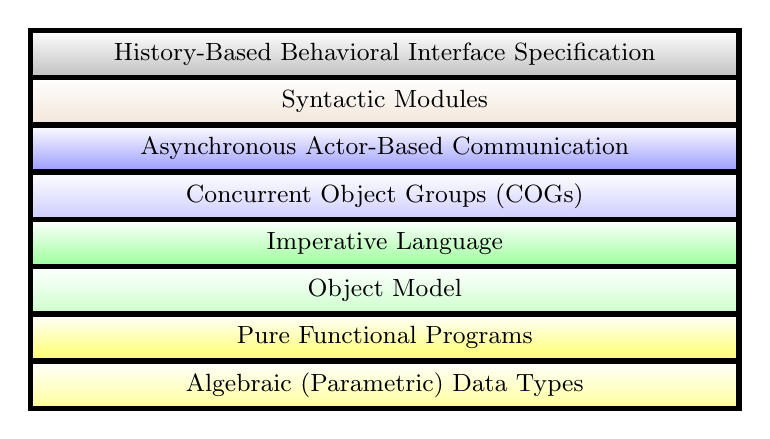
\begin{tikzpicture}[scale=1]\small
\node[rectangle, 
          ,shading=axis,shading angle=180,top color=white,bottom color=black!25, line width=2pt,
          minimum width=9cm, minimum height=.6cm, draw] (ass) at (0,4.5) 
          {History-Based Behavioral Interface Specification};

\node[rectangle, 
          ,shading=axis,shading angle=180,top color=white,bottom color=brown!20, line width=2pt,
          minimum width=9cm, minimum height=0.6cm, draw] (mod)
          at (0,3.9) {Syntactic Modules}; 

\node[rectangle, 
          ,shading=axis,shading angle=180,top color=white,bottom color=blue!40, line width=2pt,
          minimum width=9cm, minimum height=0.6cm, draw] (async)
          at (0,3.3) {Asynchronous Actor-Based Communication}; 

\node[rectangle, 
          shading=axis,shading angle=180,top color=white,bottom color=blue!20, line width=2pt,
          minimum width=9cm, minimum height=0.6cm, draw] (cog)
          at (0,2.7) {Concurrent Object Groups (COGs)}; 

\node[rectangle,
          shading=axis,shading angle=180,top color=white,bottom color=green!40, line width=2pt,
          minimum width=9cm, minimum height=0.6cm, draw] (imp) at
          (0,2.1){Imperative Language};

\node[rectangle,
          shading=axis,shading angle=180,top color=white,bottom color=green!20, line width=2pt,
          minimum width=9cm, minimum height=0.6cm, draw] (object) at
          (0,1.5){Object Model};
\node[rectangle, 
          shading=axis,shading angle=180,top color=white,bottom color=yellow!60, line width=2pt,
          minimum width=9cm, 
          minimum height=.6cm, draw] (exp) at (0,0.9) {Pure
            Functional Programs};

\node[rectangle
          ,shading=axis,shading angle=180,top color=white,bottom color=yellow!40, line width=2pt,
          minimum width=9cm, minimum height=0.6cm, draw] (adt) at
          (0,0.3){Algebraic (Parametric) Data Types};
\end{tikzpicture}
\caption{Syntax layers of the ABS language}
\label{fig:layer}
\end{figure}

\paragraph{Language description} 
In Fig.~\ref{fig:layer} the language layers of ABS are
displayed. Based on parametric (first-order) abstract data types, a
simple, pure, first-order functional language with pattern matching
and strict evaluation is defined. On top of that are objects and a
standard imperative layer. So far, this is very much like
\textsc{Scala}-light.

The central issue for achieving automated, scalable analysis is the
design of the concurrency model. Formal analysis of multi-threaded
languages with interleaving semantics, for example, \textsc{Java},
while principally possible \cite{BlomHuisman14}, is highly complex and
seems to be out of scope at the moment for relaxed memory consistency
models. To achieve feasibility, the concurrency model of ABS carefully
restricts the possible interactions among concurrent tasks while still
allowing to describe complex, realistic behavior of asynchronous
systems.  
%
More precisely, the ABS concurrency model is based on cooperative
scheduling. This means that no task is preempted (interrupted) unless
its modeler explicitly allows to do that. There are two expressions in
ABS that explicitly release control: \lstinline{release} and
\lstinline{await}. The former is unconditional while the latter has a
Boolean argument and can be used to synchronize with another task.

\begin{figure}
  \centering
\begin{lstlisting}[numbers=left,xleftmargin=4ex,escapechar=\%]
module Services;
import Data, init, modify from CustomerData;

interface Server {
  Unit process(Fut<Data> fd);
}

class Service implements Server {
  Unit process(Fut<Data> fd) {
    await fd?; %\label{abs:process:awaitd}%
    Data rd = fd.get;
    rd.modify(); %\label{abs:process:sync}%
  }
}
{ // main block
Server s = new local Service(); %\label{abs:main:begin}%
Data d = new local Data(); 
Fut<Data> fd = d!init(); %\label{abs:main:init}%
s!process(fd); %\label{abs:main:end}%
}
\end{lstlisting}  
  \caption{A simple ABS model}
  \label{fig:abs-simple}
\end{figure}

%% Besser producer/consumer?

% module Services;

% interface Server {
%   Unit produce();
%   Unit consume();
% }

% class Service implements Server {
%   Int MAX = 17;
%   Int stock = 0;
  
%   Unit produce() {
%     while (True) {
% 	  await stock < MAX;
%       stock = stock + 1;
%       }
%   }
  
%   Unit consume() {
%     while (True) {
%       await stock > 0;
%       stock = stock - 1;
%       }
%   }
% }

% { // main block
%   Service s = new Server();
%   s!produce();
%   s!consume();
% }

We explain the concurrency model of ABS with help of the code in
Fig.~\ref{fig:abs-simple}. The unit of distribution in ABS is a
\emph{concurrent object group} (COG) which can be thought of as a set
of tasks that share a common heap and a single processor. Each task
executes code owned by an object and at most one task is active in a
given COG at any time. New tasks are created by asynchronous method
calls as well as, initially, by selecting the main block of a
module. An example of the latter is the code in
lines~\ref{abs:main:begin}--\ref{abs:main:end}.

Line~\ref{abs:main:begin} declares and creates a new object with
interface type \lstinline{Server} using the implementation in class
\lstinline{Service}.  The directive \lstinline{local} places the
object in the current COG. Without \lstinline{local} a new COG is
created together with the object. The next line declares and creates a
data object (note that interface \lstinline{Data} must be imported) in
the same COG. Hence, \lstinline{s} and \lstinline{d} share the same
heap. Line~\ref{abs:main:init} calls an initialization method
(implementation not shown) on the data. The notation ``\lstinline{!}''
signifies an asynchronous call. Its effect is to create a new task in
the COG of \lstinline{d} that executes the code of
\lstinline{init()}. Asynchronous calls do not interrupt the caller, so
the statement following the call is immediately executed. Therefore,
we need a handle by which to retrieve the result of an asynchronous
call once its result has been computed. In ABS the type of such
handles have a future annotation. As can be seen in
Line~\ref{abs:main:end}, it is possible to pass futures as
parameters. This makes it possible to use the result of an
asynchronous call in different places without copying it.

After execution of the main block finished, two tasks in the current
COG are waiting, corresponding to the calls to \lstinline{init()} and
\lstinline{process()}, respectively. None of them could have started
while the main block was still executing, because there was no
synchronization expression in the latter. ABS does not determine which
of \lstinline{init()} and \lstinline{process()} is started first. In
fact, ABS can be parameterized with different scheduling
strategies. The static analyzers of ABS take all possible scheduling
sequences into account.

A first synchronisation point is reached in
Line~\ref{abs:process:awaitd} of \lstinline{process()}. It ensures
that the value of the future \lstinline{fd} is available. If
\lstinline{init()} had not been scheduled before, it will be now. Once
the value of \lstinline{fd} is available, it is retrieved with a
\lstinline{get} expression. Note that \lstinline{rd} and \lstinline{d}
might well be aliases. The standard ABS idiom for asynchronous calls
in ABS is as follows:

\begin{center}
  \lstinline{Fut<T> fx = o!m(); ... ; await fx?; T x = fx.get;}
\end{center}

In many cases \lstinline{await} and \lstinline{get} follow an
asynchronous call directly. For this common sitation the abbreviation

\begin{center}
  \lstinline{T x = await o!m();}
\end{center}

is provided which avoids the declaration of an explicit future.

Line~\ref{abs:process:sync} contains a synchronous call which is also
possible in ABS. It results in sequential behavior, i.e., yields the
processor to the callee and blocks the caller until it
returns. Obviously, here we are interested only in the side effect
that \lstinline{modify()} has. Synchronous calls are only permitted in
the COG of the caller object.

\paragraph{Degree of synchronisation} 
If one attemps to retrieve a future value that is not yet ready, this
results in blockage of its COG until the value becomes
available. Obviously, this can easily lead to deadlocks. Many
deadlocks can be avoided by guarding \lstinline{get} expressions with
an \lstinline{await} (Line~\ref{abs:process:awaitd}). Clearly, not all
deadlocks can be prevented in this manner. In practice, however,
deadlocks are easy to avoid, because synchronisation points are
explicit. In addition, ABS comes with an automated deadlock analysis
tool for ABS \cite{CGM:SoSym2014} that detects all potential
deadlocks.  An important point is that between explicit
synchronisation points (\lstinline{release}, \lstinline{await}) no
data races can occur and computations are, therefore, deterministic.

\paragraph{Degree of transparency}

ABS is an abstract language and implementation-specific aspects
including scheduling, message queueing, object representation are
hidden from the modeler. Abstract data types and interfaces can be
used to postpone detailed design decisions while still permitting
analysis of those aspects of a model that are fully specified.

\paragraph{Data sharing}

Between different COGs no data sharing is possible. The attempt to
call a method in a remote COG with a local class argument results in a
runtime error. Within the same COG all tasks have acess to a common
heap and can modify shared data. However, objects have strictly
private visibility, that is, they can only directly access their own
fields. The fields of any other objects must be accessed by explicit
method calls (getter/setter methods).

\paragraph{Formalization and semantics}

ABS has a fully formal, small step operational semantics
\cite{hats-d1.2} that permits formal soundness theorems for the
various analyses that are available for ABS. This semantics is
directly expressed in terms of rewrite rules in \textsc{Maude} format
\cite{ClavelDELMMT07} which yields a sound interpreter for ABS.

In addition there is an axiomatic semantics in the form of a program
logic~\cite{ref:key}. The behavior of interfaces and classes can be
specified by invariants over the histories of symbolic states.
Because preemption is excluded in ABS it is sufficient to establish
invariants at explicit synchronisation points and upon the termination
of methods. It is possible to prove a composition theorem for ABS
about the relation between local and global invariants
\cite{Din14fac}. This makes it possible to prove global behavioral
properties of an ABS model by (method-)local reasoning.

\paragraph{Implementation and tool support}

As ABS has been developed with the goal of being analysable, there is
a wide range of tools available. Most of them support the full ABS
language and are fully automatic. An overview of several of the tools
is available as \cite{BFH14,WongAMPSS12}.

There is an \textsc{Eclipse} plug-in that provides a development
environment for ABS and integrates most tools, see
\url{http://tools.hats-project.eu/eclipseplugin/installation.html}. An
alternative is the web-based ABS collaboratory at
\url{http://ei.abs-models.org:8082/clients/web/} which requires no
installation and also permits to try out most ABS tools.  Here is a
list of currently supported tools for ABS:

\begin{itemize}
\item editor with syntax highlighting and integrated build system,
  including compiler error location;
\item simulator/interpreter with interactive debugger;
\item visualization of ABS model execution as sequence diagram;
\item code generator backends for Erlang, Haskell, Java
  8~\cite{serbanescuNABN14a};
\item a glass box test case generator for \emph{concurrent} models \cite{AlbertAGM15};
\item a sound deadlock analysis \cite{CGM:SoSym2014};
\item a worst-case resource analysis that can be parameterized with a
  cost model for execution time, memory consumption, transmission
  size, peak cost and various other cost categories \cite{AlbertAFGGMPR14};
\item a deductive verification tool for expressive, history-based
  property specifications \cite{ref:key}
\end{itemize}


\subsubsection{ProActive and ASP}
\paragraph{General presentation}\NOTE{including the main purpose of the language}
ASP~\cite{ref:asp} is an active object programming language especially designed for
programming distributed systems. ProActive is a Java library implementing the semantics
of the ASP calculus. The language is designed taking the constraints of distributed
programming into account, and relies on RMI as the communication layer even though
another communication mechanism can be used. ProActive is intended for distribution; it
is a middleware that supports application deployment on distributed infrastructures such
as clusters, grids and clouds.Several of the design-choices of the language can be
explained by these practical concerns.

A crucial design choice of ASP and ProActive is to ensure maximal transparency for the 
programmer: active objects and futures are manipulated like usual Java objects. The 
language automatically trigger asynchronous remote invocation or synchronisation when 
needed.

Since 2010 ASP features
\emph{multi-active objects}~\cite{ref:mao} meaning that in each active object, several
threads can run in parallel, but each thread is still isolated inside a single activity. 
Such Multi-active objects feature at the same time local concurrency and global 
parallelism.

\paragraph{Language description}\NOTE{semantics; do we include a formal semantics here?}
In ASP, active objects coexist with objects that are not active. However each object is 
placed under the responsibility of an active object. An active object together with its 
service thread(s) its passive objects, and its request queue is called an activity.
Only active objects are accessible between activities. The 
objects that are not active are only accessible within an activity; if those 
objects need to be exchanged between activities, they are copied. Based on this 
clear separation, the activity is the unit of distribution. 
In ASP each thread runs inside a single activity but in the case of multi-active objects 
several threads can execute in the same active objects. 

\TODO{Do we keep the MultiASP notation or simply call it ASP?}


The language is transparent: method calls are automatically turned into asynchronous 
requests if the targeted object is a remote active object. Similarly, futures are 
implicitly created upon asynchronous calls. Futures are also transparently manipulated: 
a wait-by-necessity is automatically triggered upon an access to an unresolved future. 
In ASP, futures are first-class: they can be passed between activities. In this case, 
when the future is resolved, the result is automatically updated at all locations.

ProActive offers an API to create active objects, 
and a runtime for handling ASP features. The following is an example of ProActive program:
\lstset{
	emph={parameters,node}, 
	emphstyle=\itshape
} 
\begin{lstlisting}
T t = PAActiveObject.newActive(T.class, parameters, node);
V v = t.bar(); 	// implicit asynchronous method call
o.foo(v); 	// non-blocking operation
v.foobar(); 	// potential wait-by-necessity
\end{lstlisting}
%%% THE FOLLOWING MIGHT BE TOO DETAILLED %%%
 An active object is created using \code{newActive}, instead of the \code{new} of Java.
 The \code{newActive} primitive takes the class to instantiate, the parameters of the
 constructor, and the node on which the active object will be deployed.
 The variable \code{v} is the result of an asynchronous call; it is an
 implicit future.
% The dynamic type of \code{v} is a future that is a dynamically created subtype of 
%\code{V}. 
 When the future value is needed to continue execution, such as in \code{v.foobar()}, 
 a wait-by necessity automatically occurs if the future is not resolved. In ProActive,  
 proxies are used to handle transparently active objects and futures.
% In ProActive, when an active object is created, it is registered in the
% RMI registry delivered with Java. A local reference to this active object is also created: 
% a proxy that delegates invocations to the active object.

 The principle of the multi-active object programming model is to execute multiple
 requests of an active object in parallel, while controlling the concurrency. 
 In practice, the 
 programmer can declare which requests (i.e. which methods of the active object) can be 
 safely executed in parallel. The internal scheduler of an active objects will allocate 
 as many threads as necessary to run those methods in parallel.
  In 
 ProActive, 
  can be used through a metalanguage, based on Java annotations.  Such requests are 
  called \emph{compatible} requests. The 
 following is an
 example of multiactive object annotations in ProActive: 
 \lstset{morekeywords={@DefineGroups,@Compatible,@DefineRules,@Group,@MemberOf} }
\begin{lstlisting}
@Group(name="group1", selfCompatible=true)
@Group(name="group2", selfCompatible=false)
@Compatible({"group1", "group2"})
public class MyClass {
  ...
  @MemberOf("group1")   
  public ... method1(...) { ... }
  
  @MemberOf("group2")   
  public ... method2(...) { ... }
}
\end{lstlisting}
In this example, two groups of requests are defined, each of them holding one method. 
The two groups are declared to be compatible (so as their method, by extension). The 
\code{selfCompatible} parameter defines whether two different requests of the same group 
are allowed to run in parallel. At runtime, a ready request is automatically executed if 
it is compatible with requests that are already executing and with older requests in the 
queue (to avoid starvation). 

Without annotations, a multi-active object is a mono-threaded active object, 
without 
any local parallelism nor race condition. Its programming is extremely simple. If some 
parallelism is desired, compatibility should be declared between requests 
that can be safely interleaved and for which execution order do not matter.
The programmer can also use dynamic informations such as request parameters or object's 
state to decide which requests are compatible.
If necessary, the programmer can even use traditional low-level Java synchronisation 
primitives to make more requests compatible but this goes a little beyond the traditional 
active-object model.

%Programming with multiactive objects follows those principles:
%\begin{itemize}
%\item Without annotations, a mult-iactive object is a mono-threaded active object, 
%without 
%	any local parallelism nor race condition.
%\item If some  Compatible 
%	requests should access disjoint memory locations to avoid race conditions. Possibly, 
%	the expert programmer can also protect the access to some of the variables using a 
%	lower-level synchronization mechanism and declare more methods as compatible. 
%Generally, 
%	compatibility is statically declared but can also be decided \emph{dynamically} 
%depending 
%	on invocation parameters or on the object's state.
%\item If even more parallelism is required, an expert programmer can also protect the
%access to some of the variables using a lower-level synchronization mechanism and
%declare more methods as compatible.
%\end{itemize}
Other high-level specifications are available in multiactive
objects~\cite{henrio:hal-00916293}, such as request priority. To avoid thread explosion,
it is also possible to set a limit on the number of threads running in parallel.  The
limit can be applied in two ways: a hard limit restrains the overall number of threads
whereas a soft limit only counts threads that are not in wait-by-necessity. 
Additionally, threads can be limited per group.

As a conclusion, ASP and ProActive are based on the multiactive object programming
model.
This model is well adapted to non-expert because it provides high-level features for distribution 
and safe concurrency.

\NOTE{Below I write one paragraph on  each aspect we want to compare the language on. We 
will see later if these paragraphs stay here or are collected in another specific section}

\paragraph{Degree of synchronisation}
In ASP the only blocking synchronisation is the wait-by-necessity on a future, but the 
only way to have another thread running is to perform an invocation on an active object. 
Requests run until completion. Consequently, there is a lot of potential deadlocks in 
case of reentrant calls especially if no compatibility annotation is specified. On the 
contrary, synchronisation only occur when the future value is indeed needed and in 
particular future references can safely be transmitted between activities without 
requiring any additional synchronisation.

\paragraph{Degree of transparency}
In ASP the programmer is not explicitly exposed to the notion of future or active object 
except at active object creation. The syntax is the same as the syntax for sequential 
programming, there is no specific construct for waiting a future value or performing an 
asynchronous call. Very often a sequential code can be reused unchanged in a distributed 
setting.

\paragraph{Data sharing between threads and active objects}
ASP follows a strict policy of absence of sharing between active objects.Objects that are 
not active objects and are passed between activities (as request parameters or request 
results) are passed by copy. Of course this also applies to objects referenced by passed 
objects and a deep-copy mechanism is used ensuring that, when objects are transmitted 
between activities, they are copied as well as all their dependency on the destination 
side. This mechanism, which is the one used by RMI, slows down request invocation because 
of the time spent to transmit data, but accelerates request treatment because there is no 
need to contact another activity to get the value of the request parameters.

There is no coherency ensured between the different copies of a passive object, thus if 
the user wants to ensure that an object has a unique coherent state he should not 
transmit it by copy, and for example transmit an active-object reference instead.

\paragraph{Formal support and semantics}

Several papers formalise the semantics of ASP. The first of them formalised the 
mono-threaded part of the language and proved some determinacy 
properties~\cite{CHS:POPL04}. In particular, this paper proved that the order of future 
updates has no influence on the execution and that the only source of non-determinacy in 
mono-threaded ASP is when two activities can send a request to the same destination.
A functional fragment of the calculus has also been 
formalised in Isabelle/HOL~\cite{HKL:SCP11}. A specific semantics has been exhibited tin 
order to evaluate a functional ASP program without risk of having a deadlock; the absence 
of deadlock has been proved in Isabelle/HOL.
The full semantics of imperative ASP with multi-threaded activities is published 
in~\cite{HHI2013:mao}.

As shown in~\cite{BHR2014:gcm}, ProActive active objects, and active objects in general,
provide a convenient programming model for component based composition of distributed
applications. The ProActive library implements the GCM distributed component model. In
this context, the Vercors
platform\footnote{\url{https://team.inria.fr/scale/software/vercors/}} provides
verification capacities for ProActive components; Vercors consists of an Eclipse plugin
for designing component systems; from this point the Vercors platform can on one hand
verify the correct behaviour of the application using the CADP model-checker, and on the
other hand generate an executable ProActive/GCM corresponding to the designed system.

\TODO{do we want to put the language semantics here ?}

\paragraph{Implementation: programming and execution support}
ProActive is the Java library implementing ASP semantics. 
In ProActive, in order to transparently handle active objects and futures, a proxy is created for each of them. Proxies encapsulate all needed code to perform asynchronous, remote method invocations and wait-by-necessity behavior. Whenever an active object or a future is given as parameter of a call to an active object,  it is in fact their proxy that is copied. This way, all copies of a proxy of an active object/future points to this same active object/future. 
Another particular aspect of ProActive deals with
the deployment of ASP active objects on distributed infrastructures. The design choices of the programming language typically target a high performance of distributed ProActive applications. 
In order to settle active objects on distributed infrastructures, ProActive features a deployment specification mechanism. The goal of this mechanism is to make the physical deployment independent from the the deployment logic. This is possible by having a binding from virtual node names, used in the source code, to machine addresses or names. In practice, this binding is implemented in XML configuration files. Also, since the binding is made at \emph{deployment time}, changing infrastructure for a given ProActive application is localized in one or a few files and does not require application recompilation. 
Several machines can be aggregated under a single virtual node name in the deployment logic, for example to provide the virtual node with some properties or non functional deployment options (such as fault tolerance or logging). The deployment support of ProActive 


\subsubsection{Encore}

\section{Implementation of active objects}
A comparison of Active object language implementations based on a set of comparison 
criteria including at least:

efficient implementation of the threading model (eg for cooperative scheduling)
comparie with: old java backend;
Encore explicit bytecode operations; haskell; new java backend; ProActive?

	


\section{Lessons Learned and Conclusion}

%\section{Introduction}\label{Introduction}
%
\section{Generalities about actors and active objects}
\emph{We should probably start by  a section giving the common principles of actor and 
active object languages, giving also the vocabulary}

The active object model is  derived from the Actors
model \cite{DBLP:conf/birthday/AghaT04,agha97foundation,Agha86-book}. Actors and active objects share
a lot of concerns and advantages. A great part of the mechanisms
designed for one programming paradigm can be applied, almost
straightforwardly, to the other.


The principle of active objects is very simple: An object is said to be
active if it can be deployed on a remote machine. As a consequence,
every call to such an object will be a remote method invocation; we
call such an invocation a \emph{request}. An active object is thus an
object that treats the requests it receives, it is an object together
with a thread.

To decouple the invocation object from the invoked object, contrarily
to a classical remote invocation, the invoker is not blocked waiting
for the result instead a future object is created and represents the
result of the remote invocation.

Futures, first introduced in Multilisp \cite{Halstead85} and ABCL/f~\cite{ABCL1994}
are used as constructs for concurrency and data
flow synchronisation. Futures are language constructs that improve
concurrency in a natural and transparent way. A future represents a
result that has not been computed yet. When the result is available it
can be retrieved (automatically or manually), we then say that the
future is \emph{resolved}.
Frameworks that make use
of explicit constructs for creating futures include
Multilisp~\cite{Halstead85}, $\lambda$-calculus \cite{jlambda-fut06}, Creol
\cite{Elinar2006}, SafeFuture API \cite{SafeFutures05}, and ABCL/f
\cite{ABCL1994}. In contrast, futures are created implicitly in
frameworks like  ASP \cite{CHS:POPL04}, \cite{CHS-IC2008},
\cite{CH-book},
AmbientTalk~\cite{DedeckerCMDM-ecoop06},
ProActive~\cite{CDD:CMST06}.  Usually, in those object-oriented languages,
implicit creation corresponds to asynchronous method invocation. A key
benefit of the implicit creation is that no distinction is made
between synchronous and asynchronous operations in the program.
This way, when a method invocation is local, usual method invocation
is performed, whether when the accessed object is remote, a future is
immediately obtained.

Additionally, the futures can be accessed explicitly or implicitly. In
case of explicit access, operations like \emph{claim} and \emph{get},
\emph{touch} are used to access the future \cite{Elinar2006,ABCL1994}.
For implicit access, operations that need the real value of an object
(\emph{blocking} operations) automatically trigger synchronisation
with the future update operation. We say that futures are \emph{first
	class} if future references can be transmitted between remote
entities without requiring the future to be resolved.



\section{Criteria for comparison}
\emph{Here we suggest to summarise the points of comparison between different active 
object languages}


The principle of active objects is to associate a thread to an object, or to a set of
objects. We call \emph{activity} this notion: a thread and the objects
managed by this thread.  Two objects in different activities 
communicate by remote method invocation: when an object invokes a
method on an object in another activity, this creates a
\emph{request}; the invoker continues its execution while the invoked
object will serve the request in an asynchronous manner. Requests wait for execution in a \emph{request queue}. Like in any
object-oriented language, method invocations can return results. In
order to allow the invoker to continue its execution, a placeholder
for the expected result must be created. \emph{Futures} play this
role: a future is an empty object that will later be filled by the
result of a request. We say that a future is \emph{resolved} when its
value is known.
Overall, the active object paradigm makes programming of distributed
applications more natural, especially when applications are made of
computational entities that may have a state like objects, and that
execute in a decoupled manner because they are distributed.
While all active object models rely on the previously introduced notions, their
detailed characteristics vary in practice, which we present below:

\subsubsection{How are objects associated to activities?}\label{sec:activity}
We distinguish three different ways to map objects to threads/activities: 
\begin{itemize}
	\item \textit{Uniform Object Model.}  All objects are active objects
	with their own request queue and their own private execution thread.
	In consequence, all communications between objects occur by posting
	a request. This model is simple to formalise but its implementation
	is more difficult as it must rely on the creation of logical thread
	to allow scalability.
	\item \textit{Non Uniform Object Model.}  Some of the objects are not
	active, in which case they are only accessible by a single active
	object, they are part of its state. 
	An activity contains one active and several passive objects. Non-uniform active object models
	are much more efficient as they require less communications and
	less concurrent threads than models where each object would be
	active. Reducing the number of activities also reduces the number of
	references that are globally accessible in the system, and thus enables the
	instantiation of a large number of objects.
	\item \textit{Object Group Model.}
	In this model, an activity is made of a set of objects sharing a
	request queue and an execution thread, but all
	objects can be invoked from another activity. This
	approach improves scalability as it reduces the number of threads, but
	it is still difficult to create a lot of objects as all of them must
	be registered so that they are accessible from any other activity.
\end{itemize}

\subsubsection{How are requests scheduled?}
We distinguish three  threading models in active object languages.
\begin{description}
	\item \textit{Single-threaded.} 
	Within an active object, requests are executed sequentially without
	interleaving possibilities. 
	\item \textit{Cooperative scheduling.}
	A running request can explicitly release the execution thread to let
	another request run. Requests are not processed in parallel but they
	might interleave. Data-races are avoided.
	\item \textit{Multi-threaded.}
	Within an active object, requests are executed in parallel using
	different threads, without pausing nor yielding.
	Some data-races inside the activity is possible. This is
	called a \emph{multiactive object} model.
\end{description}

\subsubsection{Is the programmer aware of distributed aspects?}
Some active object languages use a specific syntax for asynchronous
method calls: a different operator is used to distinguish them from
synchronous method calls. This makes the programmer aware of the
places where futures are created. Generally, when asynchronous
invocation is explicit, there exists a special type for future objects.
Additionally, the futures, when they are statically identified, can be
accessed explicitly or implicitly. In case of explicit access,
operations like \emph{claim}, \emph{get} and \emph{touch} are used to
access the future. This is particularly convenient for releasing the
current thread if a future is not available in case of cooperative
scheduling (\emph{await} statement). For implicit access, operations that need the real
value of an object (\emph{blocking} operations) automatically trigger
synchronisation with the future update operation.
Implicit future creation allows transparency of distributed aspects:
there is almost no difference between a distributed program and usual
objects, whereas explicit manipulation of futures allows the
programmer to better control its execution, but requires from him a
better expertise. We say that futures
are \emph{first class} if future references can be transmitted between
remote entities without requiring the future to be resolved.





\section{Active object and Actor languages}\label{sec:overview}
\emph{Here we suggest to have a list of active object languages referring to the 
preceding classification}

Several programming languages or models rely on some form of active
objects, we review the main ones below. Especially focusing on
languages which have a formalised semantics. But before focusing on
active objects, let us first review the main works on formalisation of
futures in the context of functional languages.
Indeed, Futures
were first introduced in Multilisp \cite{Halstead85}, and thus lead to
a lot of work on their formalisation in the context of 
functional languages. We will then review main active object languages
and finish by a couple of languages that are not pure active objects
but also strongly relate the notions of distribution and concurrency to
the notion of objects.



\subsection{Futures in functional languages}
To our knowledge, the first work on formalisation by semantic rules of
Futures appeared in \cite{FlanaganFelleisen99,FlanaganFelleisen1995} and was intended at
program optimisation. This work focuses on the futures  of MultiLisp,
that are explicitly created. The authors ``compile'' a program with
futures into a low-level program that does explicit touch operations
for resolving the future, and then optimise the number of necessary touch operations.

In a similar vein,
$\lambda(fut)$ is a concurrent lambda calculus with futures.
It features non determinism primitives (cells and handles). In
\cite{jlambda-fut06}, the authors define a semantics for this calculus,
and two type systems. They use
futures with explicit creation point in the context of $\lambda$-calculus; much in
the same spirit as in Multilisp. Alice~\cite{Niehren:Sabel:Schmidt-Schauss:Schwinghammer:06} is an
ML-like language that can be considered as an implementation of
$\lambda(fut)$.



\subsection{Asynchronous Sequential Processes}
The ASP calculus we have defined~\cite{CH-book} is a distributed active object calculus with futures;  the
ProActive library \cite{CDD:CMST06} can be considered as its reference
implementation.  The ASP calculus formalises the
following characteristics of active objects:
\begin{itemize}
	\item \emph{asynchronous communications}, by a request-reply mechanism;
	\item \emph{futures}; in ASP, futures are transparent
	objects: their creation and access is implicit, futures are also
	\emph{first-class}: they can replace
	transparently any other objects and can be communicated as 
	result or parameter of remote method invocations;
	\item \emph{sequential execution} within each process, each object
	is manipulated by a single thread;
	\item \emph{imperative objects}, i.e. each object has a state and
	there is an operation for updating it.
\end{itemize}

ASP's active objects are quite similar to actors and ensure the
absence of sharing: objects live in disjoint activities. An activity
is a set of objects managed by a unique process and a unique
active object.  Active objects are accessible through global/distant
references.  They communicate through asynchronous method calls with
futures. 
ASP is a non-uniform active object model: some of the objects are
not active, in which case they are only accessible by a single active
object, they are part of its state. Non-uniform active object models
are much more efficient as they require much less communications and
much less concurrent threads than models where each object would be
active.

Our main result consists in a confluence property and its
application to the identification of a set of programs behaving
deterministically.  This property can be summarised as follows:
\begin{itemize}
	\item 
	Future updates can occur at any time without any consequence on the
	result of the computation,
	\item Execution is only characterised by the order of requests, and
	even more precisely by the order of request senders: To characterise
	uniquely an execution,
	it is sufficient to consider, for each activity, the ordered list
	of identifiers of the activities that have sent a request to this activity.
	\item Consequently, programs communicating over trees are deterministic.
\end{itemize}


The code snippet shown in Figure~\ref{fig:pasniplet} gives a typical
example of a simple ProActive piece of code. It
creates a new active object of type \code{A} on the JVM identified
by \code{Node1}. All calls to that remote object will be
asynchronous, and the access to the result might be subject to \emph{wait-by-necessity}.
% \begin{small}
\begin{figure*}[t]
	\begin{lstlisting}[frame=single]
	A a = (A) ProActive.newActive("A", params, Node1); // active object creation
	v = a.bar (...);   // Asynchronous call, no wait, v gets a future
	o.gee (v);         // No wait, even if o is a remote active object and v is still awaited
	...
	v.f (...);        // Wait-by-necessity: wait until v gets its value
	\end{lstlisting}  % \end{verbatim}
	\caption{Typical ProActive code}
	\label{fig:pasniplet}
\end{figure*}% \end{small}

\smallskip

The main advantage of ASP is that most code can be written without
caring about distribution and concurrency.  Futures are automatically
and transparently created upon method invocation on an active object.
Synchronisation is due to wait-by-necessity that occurs
upon access to a future that has not been resolved yet.
This synchronisation is performed transparently, i.e. 
there is no  construct for explicitly waiting the result of
a request. Wait-by-necessity is always
performed at the last moment, i.e. when a value is really needed.
Futures are also transparently sent between activities. This
way simple programs can be written extremely easily and rapidly.


Recent works tend to introduce local concurrency either at the actor
level
\cite{Scholliers:2014:PAM:2563745.2564410,ref:spec-actors} or at the
active object level, in particular with multiactive objects
\cite{ref:mao}.
Multiactive objects avoid deadlocks that are likely to arise
%when doing reentrant calls 
with mono-threaded active objects, and take
advantage of multi-core architectures.  
%The principle of multiactive objects is to execute
%multiple requests of an active object in parallel, while controlling
%the concurrency.
%The multiactive object model has been implemented as an extension of ProActive. This 
%extension comes as a small metalanguage to allow 
In practice, a programmer declares which requests of an active object can safely be
executed in parallel, namely which requests are \emph{compatible}. An implementation of 
multiactive objects is available in the latest version of ProActive; 
%The
%metalanguage to do that in ProActive 
it is based on the Java annotation
mechanism:
% A programmer can use these annotations on top of a class so that all objects of this 
%class are automatically multiactive objects when instanciated with the \code{newActive} 
%ProActive primitive\footnote{if there is no annotation, then objects crerated with the 
%\code{newActive} primitive remain basic active objects}. 
%Request compatibility can be specified following three steps:
%\begin{itemize}
%\item A programmer first uses the \code{@Group} annotation on top of a class to define a 
%group of requests. A group is meant to gather requests that have the same concerns 
%and/or 
%the same compatibility requirements. 
%\item Then, a programmer uses the \code{@MemberOf} annotation on top of a method 
%definition to make this method belong to a particular group (previously defined).
%\item Finally a programmer uses the \code{@Compatible} annotation to specify which group 
%is compatible with which other group, so, in extension, to specify which requests can be 
%run in parallel safely. 
%\end{itemize}
%Below is an example of an annotated
%class \code{MyClass}:
%\ttfamily\scriptsize
\setlength\abovecaptionskip{0.25mm}
\lstset{
	morekeywords={@DefineGroups,@Compatible,@DefineRules,@Group,@MemberOf},
} 
\begin{lstlisting}
@Group(name="group1", selfCompatible=true)
@Group(name="group2", selfCompatible=false)
@Compatible({"group1", "group2"})
public class MyClass {
...
@MemberOf("group1")   public ... method1(...) { ... }
@MemberOf("group2")   public ... method2(...) { ... }
}
\end{lstlisting}
In this example, groups of requests are defined with \code{@Group} and filled with
\code{@MemberOf}. Group compatibilities are specified with
\code{@Compatible}. Parameter \code{selfCompatible} defines
whether two different requests of the same group are allowed to run in
parallel.  Upon execution, a ready request is executed if it is
compatible with requests that are executing and with older
requests in the queue to avoid starvation.  


It is also possible to set a limit on the number of threads running in
parallel~\cite{henrio:hal-00916293}.  The limit can be applied in two ways: a hard limit
restrains the overall number of threads whereas a soft limit only counts threads that are
not in wait-by-necessity.  Additionally, threads can be limited per group.

Multiactive objects enable high-level implementation of scheduling policies. We use their 
features to implement the ProActive backend for ABS.


\subsection{AmbientTalk}
In AmbientTalk \cite{DedeckerCMDM-ecoop06}, there is one major difference compared to the 
other active-object models presented above: in AmbientTalk the future access is a
non-blocking operation, it is an asynchronous call that returns
another future.  There is no wait-by-necessity upon a method call on a
future, instead the method call will be performed when the future
becomes available, in the meantime a future represents the result of
this method invocation.  This differs from the approach adopted in
other frameworks where access to a future is blocking.  This approach
avoids the possibility of a deadlock as there is no synchronisation,
but programming can become tricky.
Overall, two activities can only coordinate through  callbacks.  This
inversion of control has the advantage to avoid deadlocks but breaks the program into
independent procedures where sequences of instructions are difficult to enforce.



\subsection{Creol} Creol \cite{Johnsen2006a,Elinar2006} is an active object language
that executes several requests at the same time, with only one active at a given time.
This is some form of \emph{collaborative multi-threading} based on an \emph{await}
operation that releases the active thread so that another request can continue its
execution. Typically, one would do an \emph{await} when accessing a future so that if
the future is not yet available another thread can continue its execution. In Creol
\cite{Johnsen2006a} future creation and access is explicit, in particular a specific
syntax exists for asynchronous method invocation. Creol is a uniform active object model
where each object is an active one able to receive remote method invocations.  Creol
also ensures the absence of data races, even if request execution can be interleaved,
and the result of computation is less predictable than in pure mono-threaded active
object models.


De Boer et al.   \cite{SDE:BoerCJ07}  provided 
the semantics of an
object-oriented language based on Creol; it features
active objects, asynchronous method calls, and futures. This semantics
extends Creol in the sense that it
supports first-class futures, although the future access is  still
explicit (using \emph{get} and \emph{await}). 
In the same paper, the authors also provide a proof system for proving properties
related to concurrency. 

\smallskip


Overall, explicit future access,
explicit release points, and explicit asynchronous calls make the Creol
programming model rich, but also requires more expertise from the programmer than the 
languages featuring more transparency. 


\TODO{probably move next paragraph} The cooperative multithreading model has the
advantage of having less deadlocks than mono-threaded active objects, because in
mono-threaded models like ASP a request must be finished before addressing the next one.
Indeed, when the result of a request is necessary in order to finish another one, the
Creol programmer can release the service thread, which is impossible in mono-threaded
models. In particular, accessing futures can lead to deadlock in case of re-entrant
requests. While no data race condition is possible, interleaving of the different
request services triggered by the different release points makes the behaviour more
difficult to predict (in particular the determinism properties of ASP cannot be proven
in Creol).
 The partial solution proposed by ASP and ProActive is ``first-class
futures'': since futures are implicitly created and transparently
transmitted as method parameters and results, the deadlock only occurs
if the future is really needed.  Alternatively, Creol, ABS, and JCoBox
provide explicit futures and allow the active thread to suspend itself
until a result is returned. Multi-active objects also allow an object to serve a 
re-entrant request provided it is compatible with the other ones.

\subsection{JCoBox}
JCoBox \cite{schafer2010jcobox} is an active object programming model
implemented in a language based on Java.  It integrates asynchronous
and synchronous communications as different operators, and partitions the
object space into ``coboxes'', similar to ASP's
activities. Each cobox is responsible for controlling the local
concurrency and maintaining its invariants. 
%Like in Creol, in each cobox, a single
Similarly to Creol, in each cobox a single thread is active at a time, but this thread can be released and coboxes
support collaborative multi-threading.


In Creol \cite{Johnsen2006a} all objects are active, whereas ASP
and JCoBox are non-uniform active object models: some objects are active and are invoked by asynchronous
remote requests, other objects are passive and are accessible by a
single activity (or cobox), they are transmitted by value.  References
from a cobox to an active object of another cobox are called ``far
references''. Far references can only be used to perform asynchronous
calls (\code{reference!method()}), which return futures.  Futures are
explicitly created and explicitly accessed, just as in Creol.
\code{await} performs a cooperative wait on the future, whereas
\code{get} blocks until the value of the future is received.  In
JCoBox,  a cobox may contain multiple active objects.

Cooperative multi-threading is similar and leads to the same
advantages and drawbacks as  in Creol. 


 



\subsection{JAC}

JAC \cite{lohr2006jac}  is an extension of Java that introduces a
higher level of concurrency and separates thread synchronisation from
application logic in a declarative fashion. JAC relies on a custom
pre-compiler and declarative annotations, in the form of Javadoc
comments placed before method headers or inside the code. Objects are
annotated as \code{controlled} when their threads are managed and
synchronised according to JAC's annotations. JAC relies on
compatibility annotations stating whether two methods can be executed
at the same time; two methods should be compatible if they do not
access the same variables (or if the access to those variables has
been protected by some locking mechanism).  For example, the following
code states that \code{isEmpty} can be safely executed concurrently
with \code{lookup} and with itself:
\begin{lstlisting}
/** @compatible lookup(Object), isEmpty() */
public boolean isEmpty() {.....}
\end{lstlisting} 

This way methods that can safely be run concurrently will
automatically be. Additional annotations are given for finer grain or
easier control of concurrency and synchronisation (e.g. to wait for a
guard to be verified before executing a method).  Exhaustive case
study of annotation effect, in particular in relation with inheritance
is also described in \cite{lohr2006jac}.

JAC's \emph{async} annotation provides some form of
active object behaviour: an asynchronous method is executed
independently of others in a separate thread. The main difference with
classical active objects is that classical active objects act as a unit of
concurrency: they are manipulated with a single thread and enforce the
absence of shared memory between active objects. Stating that all
methods of a class are asynchronous and mutually exclusive would
create some form of active objects, but without the absence of shared
memory enforcement. For example, in ASP and JCoBox, non-active objects
are called passive and are deeply copied when passed between
activities in order to guarantee the absence of sharing.

\smallskip We think JAC is a well designed model for declaring simply
powerful concurrency rules, but unfortunately it is not particularly
adapted to a distributed environment. Classical active objects on the
contrary provide a better encapsulation of data and concurrency but do
not provide concurrency abstractions as powerful as JAC annotations.
This way to annotate programs for concurrency is quite similar to multi-active objects 
featured by ASP, but the fact that ASP annotations are restricted to compatibility of 
requests makes it much less expressive but much simpler to use.

% \begin{figure*}[t]
% \begin{lstlisting}[frame=single]
% public class Peer {
% ...
% /** @when !runningAdd
% */
% public JoinResponse join(Peer other) { 
%   runningJoin = true;
%   //do logic
%   runningJoin = false;
% }

% /** @compatible add(Key, Serializable), join(Peer)
%     @when !runningJoin || !inSplittingZone(k)
% */
% public void add(Key k, Serializable value) { 
%   runningAdd = true;
%   // do logic
%   runningAdd = false;
% }

% private boolean inSplittingZone(Key k){ ... }

% }
% \end{lstlisting}
%  \caption{The CAN Peer implemented in JAC \TODO{CHECK: what happens if
%    the setting of flags interleaves??? is this example even possible
%    in JAC without side effects in guards or scheduler?? hOW???}}
%  \label{jac_can_peer}
% \end{figure*}

% In  our opinion multi-active objects 
% offer a simpler annotation system and a higher synchronization logic encapsulation 
% for the  programmer. On the other hand, JAC's inheritance model is
% well designed and resembles the  way our
% annotations are inherited on from class to class.



\smallskip\noindent\textbf{ABS.}\label{abs}
ABS~\cite{ref:abs} is an object-oriented programming language based on active objects that targets
modelling of distributed applications. ABS syntax is based on classes.
ABS has an object group model
based on the notion of concurrent object
group (hereafter named COG). 
%Object fields can only be accessed within the object methods. 
Asynchronous method calls and futures are explicit as in the following example:
%, and there is not yet support for first class futures.
% The following example is an asynchronous call that returns a future of
%parametric type \code{V}:
\lstset{frame=single} 
\begin{lstlisting}
Fut<V> future = object!method();
\end{lstlisting}

Requests are scheduled in a cooperative manner once again thanks to the \code{await} keyword, used as follows:
% that can be followed by a future or a condition, as in the two following examples:
\lstset{frame=single,
	morekeywords={await}}
\begin{lstlisting}
await future?;
await a > 2 && b < 3;
\end{lstlisting}
In those examples, the execution thread is released if the future is not resolved or if the condition is not fulfilled. 
%In those cases, the execution thread is handed over to another ready request. 
%A paused request is ready to resume when the future is resolved (in \code{case ~1}) or when the condition is fulfilled (in \code{case ~2}).
ABS also features a \code{get} accessor to retrieve a future's value; it blocks the execution thread until the future
is resolved: 
\lstset{frame=single,
	morekeywords={get}}
\begin{lstlisting}
V v = future.get;
\end{lstlisting}	
%The \code{get} accessor  % (and does not release the execution thread until then).
The ABS tool
suite\footnote{http://tools.hats-project.eu/} provides a wide variety of static verification engines that help
designing safe distributed and concurrent applications. Those engines
include a deadlock analyser \cite{CGM:SoSym2014}, a resource and cost analyser for cloud environments 
\cite{SACO:TACAS14,ABSresourcescost}, and general program properties verification with the ABS-Key tool~\cite{ref:key,ref:noc-abs-key}.
The ABS tool suite also includes a frontend
compiler and several backend translators into various programming
languages (Java, Haskell, Maude). 
The Java backend for ABS translates ABS programs into Java programs but is not able to
generate code that runs in a distributed manner.
%, neither in the ABS language itself nor in any of the existing backend.



\subsection{X10} 
X10 \cite{charles2005x10} is a programming language that adopts a
fairly new model, called partitioned global address space (PGAS). In this model,
computations are performed in multiple places (possibly on various computational units)
simultaneously. Data in one place is accessible remotely, and is not movable once
created. Computations inside places are locally synchronous, but inter-place activities
are asynchronous. This decouples places and ensures global parallelism. While this model
seems fundamentally different from active objects, both can be used to express the same
kind of applications, but more importantly in X10 like in ProActive, a special care has
been put to offer to the programmer a wide set of so called \emph{technical services}.
Technical services are non-functional features that are crucial to deploy and run
large-scale applications, they typically include fault-tolerance, security, code
migration, deployment on a wide set of architectures, support for several communication
protocols, etc. 

\subsection{Encore}
To be written


\section{Comparing languages} 

\emph{Here we should speak about point-to-point comparisons and every point of
	comparison that was not mentioned in the preceding section. Translation from ABS to 
	ASP is a typical example of what we want to put in this section.}

\TODO{Perhaps also fit some usecases here especially if they have been implemented using 
different models}


\section{Lessons learned and Perspectives}
\emph{Here it would be interesting to have a higher view of lessons learned, on what AO 
language to use to do what. As a perspective perhaps give the characteristics of the 
ideal active object language (can we mix some of them to make a better one?)}
%\section{Conclusion}\label{conclusion}

% Appendix
%\appendix
%\section*{APPENDIX}
%\setcounter{section}{1}
%In this appendix,...

%\appendixhead{ZHOU}

% Acknowledgments
%\begin{acks}
%The authors would like to thank Dr. Maura Turolla of Telecom
%Italia for providing specifications about the application scenario.
%\end{acks}

% Bibliography
\bibliographystyle{ACM-Reference-Format-Journals}
\bibliography{2015-active-objects-survey,biblio,envisage}
                             % Sample .bib file with references that match those in
                             % the 'Specifications Document (V1.5)' as well containing
                             % 'legacy' bibs and bibs with 'alternate codings'.
                             % Gerry Murray - March 2012

% History dates
%\received{February 2007}{March 2009}{June 2009}

% Electronic Appendix
%\elecappendix

%\medskip

%\section{This is an example of Appendix section head}

\end{document}
% End of v2-acmsmall-sample.tex (March 2012) - Gerry Murray, ACM



%%% Local Variables:
%%% mode: latex
%%% TeX-master: t
%%% End:
